%!TEX root = mainfile.tex

\section{Introduction} % (fold)
	\label{sec:introduction}

% section introduction (end)

\section{Tomographic Reconstruction} % (fold)
	\label{sec:tomographic_reconstruction}
	Tomographic reconstruction involves the creation of an image of an object taken through a particular slice by recombining the data collected from a set of line integrals across that object in the plane of interest. The word tomography comes from the Greek \textit{tomos} meaning section and \textit{graphein} meaning to write, so tomography is simply writing `parts' of an object, in this case an image of a single plane through that object, in a useful form.

    In order to examine this method of image construction, we shall use a series of images which form \textit{sagittal} slices of a human head. This means that each of the 129 images in the collection are a slice from side to side at a slightly different position. Together, they form a 3 dimensional image of the head, with all of the interior detail maintained. A few of these images are shown in figure~\ref{fig:example_sagittal}
    \begin{figure}[ht]
        \centering
        \begin{minipage}[c]{0.19\linewidth}
            \centering
            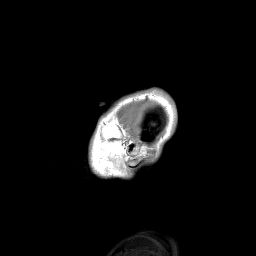
\includegraphics[width=\textwidth]{Files/report_images/sagittal_example1.jpg}
        \end{minipage}
        \begin{minipage}[c]{0.19\linewidth}
            \centering
            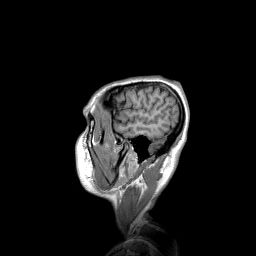
\includegraphics[width=\textwidth]{Files/report_images/sagittal_example2.jpg}
        \end{minipage}
        \begin{minipage}[c]{0.19\linewidth}
            \centering
            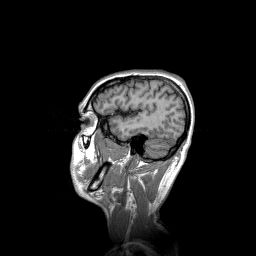
\includegraphics[width=\textwidth]{Files/report_images/sagittal_example3.jpg}
        \end{minipage}
        \begin{minipage}[c]{0.19\linewidth}
            \centering
            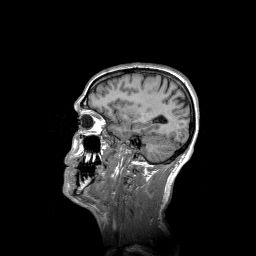
\includegraphics[width=\textwidth]{Files/report_images/sagittal_example4.jpg}
        \end{minipage}
        \begin{minipage}[c]{0.19\linewidth}
            \centering
            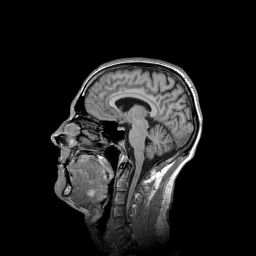
\includegraphics[width=\textwidth]{Files/report_images/sagittal_example5.jpg}
        \end{minipage}
        \caption{Example slices from the original sagittal 3D image that will be used to examine the tomographic reconstruction method. Out of the 129 images that make up the full image, these are, from left to right, image 20, 31. 38, 48 and 64 respectively.\label{fig:example_sagittal}}
    \end{figure}

    In order to demonstrate the tomographic reconstruction method as used in medical applications, an effective CT scan can be taken of this 3D image by converting it to axial slices. These are slices taken laterally through the object from top to bottom. Again, a selection of this new 3D image is shown in figure~\ref{fig:example_axial}.
    \begin{figure}[ht]
        \centering
        \begin{minipage}[c]{0.3\linewidth}
            \centering
            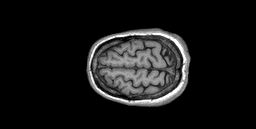
\includegraphics[width=\textwidth]{Files/report_images/axial_example1.jpg}
        \end{minipage}
        \begin{minipage}[c]{0.3\linewidth}
            \centering
            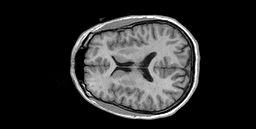
\includegraphics[width=\textwidth]{Files/report_images/axial_example2.jpg}
        \end{minipage}
        \begin{minipage}[c]{0.3\linewidth}
            \centering
            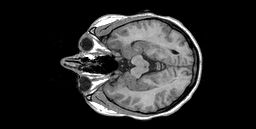
\includegraphics[width=\textwidth]{Files/report_images/axial_example3.jpg}
        \end{minipage}

        \begin{minipage}[c]{0.3\linewidth}
            \centering
            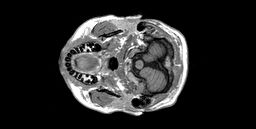
\includegraphics[width=\textwidth]{Files/report_images/axial_example4.jpg}
        \end{minipage}
        \begin{minipage}[c]{0.3\linewidth}
            \centering
            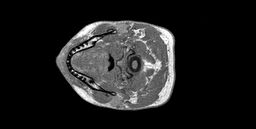
\includegraphics[width=\textwidth]{Files/report_images/axial_example5.jpg}
        \end{minipage}
        \begin{minipage}[c]{0.3\linewidth}
            \centering
            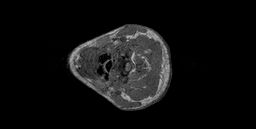
\includegraphics[width=\textwidth]{Files/report_images/axial_example6.jpg}
        \end{minipage}
        \caption{Example slices from the original sagittal 3D image that will be used to examine the tomographic reconstruction method. Out of the 129 images that make up the full image, these are, from top left to bottom right, image 78, 106, 126, 162 and 182 respectively.\label{fig:example_axial}}
    \end{figure}

    In order to show the effectiveness of the different techniques used in tomographic reconstruction, we shall refer back to a single of these slices, which will be the one that shall be reconstructed. This reference image will be image NUM out of the 256 stack above, and is shown in figure~\ref{fig:reference_slice}.
    \begin{figure}[ht]
        \centering
        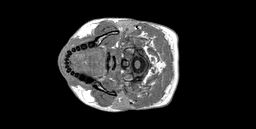
\includegraphics[width=0.4\textwidth]{Files/report_images/reference_slice.jpg}
        \caption{Example slices from the original sagittal 3D image that will be used to examine the tomographic reconstruction method. Out of the 129 images that make up the full image, these are, from top left to bottom right, image 78, 106, 126, 162 and 182 respectively.\label{fig:reference_slice}} 
    \end{figure}
    
% section tomographic_reconstruction (end)

